% !TeX root = ../main.tex
% Add the above to each chapter to make compiling the PDF easier in some editors.

\chapter{Related Work}
This master thesis focuses on two broad topics, sound and collaboration, which puts at the intersection of the fields of \gls{hci}, \gls{vr}, and \gls{cscw} and \gls{cve}. We will start with introducing the field of \gls{hci}, and the role human factors play in it.

\paragraph{HCI}
\cite[Chapter~4.1.1]{jr_3d_2017} define \gls{hci} as "a field that seeks to understand the relationship between human users and digital technological artifacts and to design new, effective ways for humans to use computer technologies for all sorts of purposes". The word "computer" can mean anything from a smartphone to a desktop computer to a \gls{vr} setup, which also implies different interfaces: touch-based, 2D, immersive 3D, etc. Modern \gls{hci} deals not only with the human-computer interactions, but also pays attention to the computer as a medium for collaborative work, and hence human-human interactions. The goals pursued by the research in the field is not to simply understand the interactions we already use today, but to design the new interactions, be it through novel hardware and software solutions or innovative application of the existing ones. Lately,\gls{hci} experienced a shift from focusing on the \gls{ui} to the \gls{ux}, which encompasses \gls{ui}, but also deals with the ecology that the system exists in (social context, cultural differences, skills and emotional state of the users, and so on).

\subparagraph{Human Factors}
One of the principal reference points in \gls{hci} is the notion of human factors, or as they are also called, ergonomics. Two of the main factors are Perception and Cognition, they constitute a significant part of this thesis, and we will now explore why that is the case. The third main factor is Physical Ergonomics, which is employed to design comfortable and effective interfaces with regard to the human physiology. It is not highly relevant for this work, and thus will be addressed only scarcely. A review of physical ergonomics factor can be found in \cite[Chapter~3.5]{jr_3d_2017}.

% 3.1 Intro: definition and examples

% 3.2 Information processing: how human IP is tied with the main human factors, the graph; short, one-paragraph, explanation of everything in the graph
If we consider the interactions with the outside world, everything we do happens based on the information we get from our environment and body. \cite{jr_3d_2017} argue that the processing of this information can be mapped to the aforementioned as humans, process this information is governed by the aforementioned human factors (see Fig. \ref{fig:informationprocessingloop}).
First, the outside events or stimuli are perceived (interpreted and understood according to past experience) through the senses. Based on the interpreted information, an action can be taken, or this information can be saved in the working (short-term) memory. Short-term memory has limited capacity, and is directly affected by the attention. Contrary, long-term memory is vast, is not directly affected by the attention, and used to store information about the world. Based on the actions taken, the responses can be fed back into the information processing loop.

\begin{figure}
	\centering
	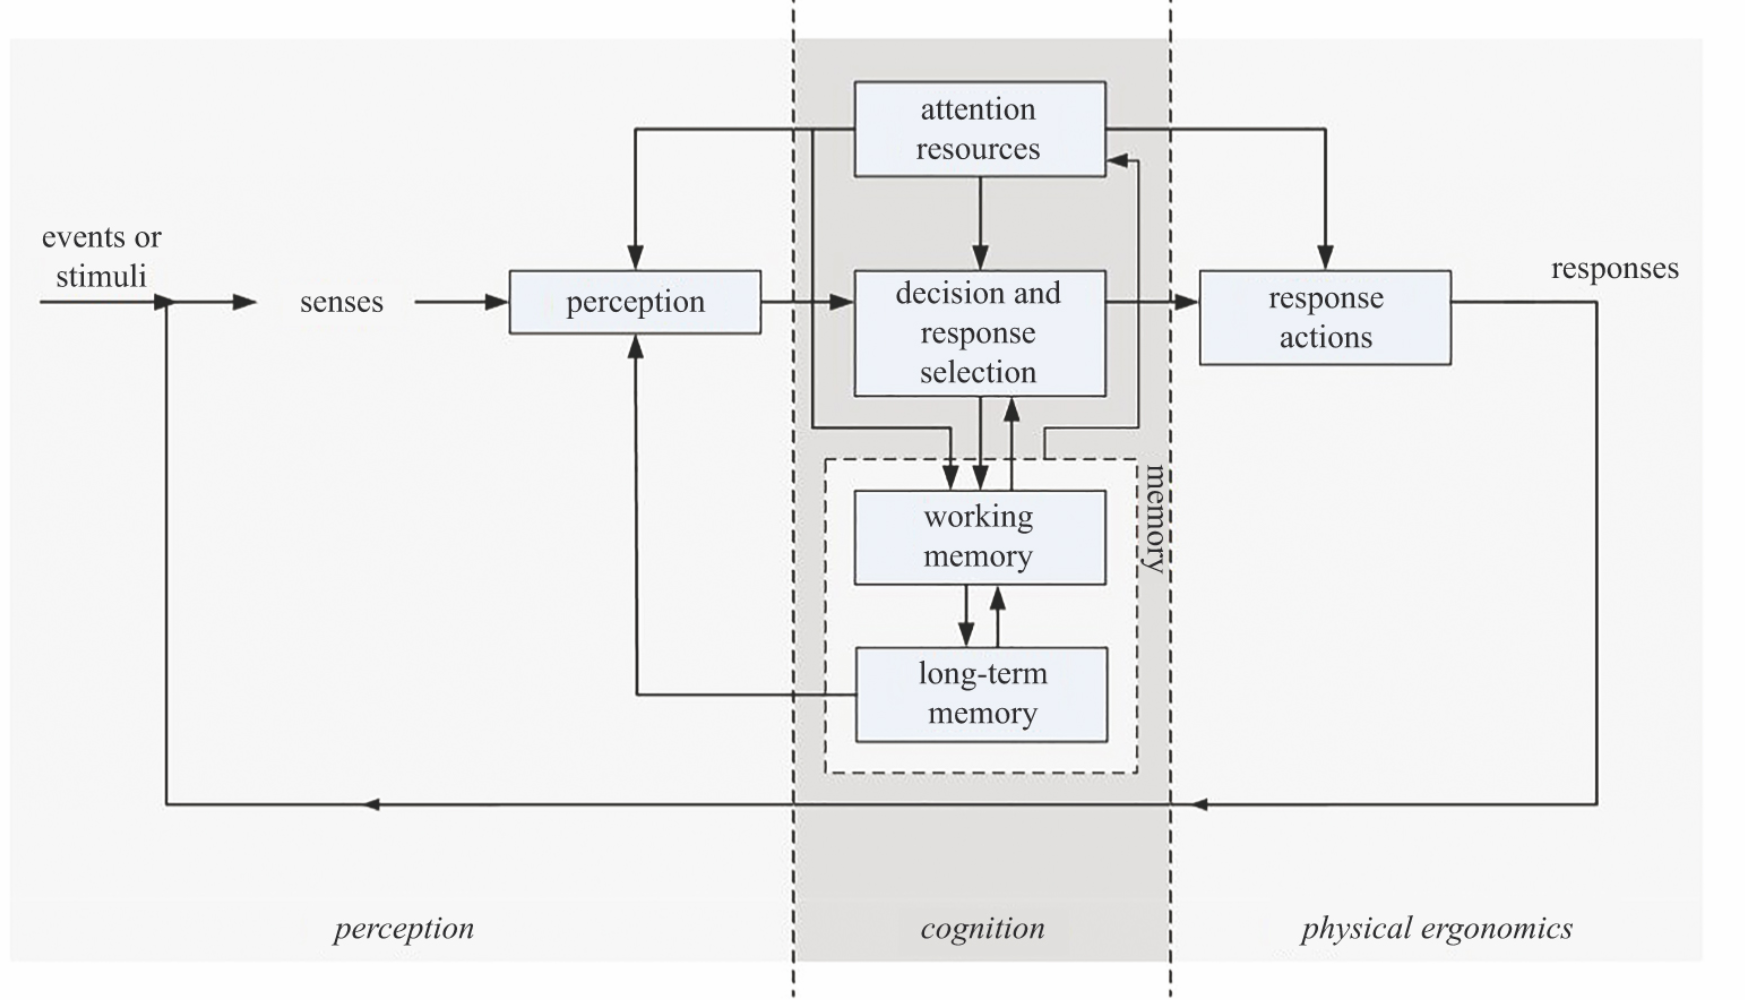
\includegraphics[width=0.7\linewidth]{figures/placeholders/information_processing_loop}
	\caption{Information processing loop (Redrawn from \cite{jr_3d_2017})}
	\label{fig:informationprocessingloop}
\end{figure}

% 3.3 Perception: responsible for auditory perseption and comprises one part of this work (perceptual mechanisms; types of perceptual cues; sensory substitution and multisensory processing)
Perception factors deal with all information, available to us through our senses: visual, auditory, somatosensory (haptic) and chemical sensing systems. This factor is responsible for receiving and interpreting information.
Previously, we hypothesized that additional auditory cues may lead to an overall improvement of the satisfaction with the collaboration experience. Auditory cues is a topic residing in the realm of perception - sounds have to be first heard and matched to the previous experience and memory. 
Additionally, the study of perception includes the topics of multisensory processing, where sensing registering an event in one sensory channel helps improve its perception in another, and of sensory substitution, where one sensory system assumes the role that would normally be taken by another (for example, the substitution of somatosensory information with sound in systems, where haptic feedback is not available).

% 3.4 Cognition governs awareness, a state of noticing certain details about the environment, people, or tasks.
Cognition is defined in \cite[Chapter~3.4] as "the driving force behind the generation and usage of knowledge". It is responsible for our thought process and is directly linked to the perception and attention. The study of cognition is a study of how these thought processes function and how cognition effects our interactions with the environment.
For the purpose of this thesis, we are interested in the concept of awareness, which focuses on the analysis and design of systems in a way that helps users be more aware of certain details about the environment (for example, other people, tasks, or the workspace).
The main cognition problems that occur in the designed interface are mental (cognition) load and human error. The former can occur due to the properties of the task (difficulty, priority, etc.), or exceeding the attention and processing resources of an individual. The latter can be generally described as a lack of success in performing the task, and can also occur due to perception and physical ergonomics issues.

% 3.5 Physical ergonomics: "enables us to design systems that can be used comfortably and effectively". Not strictly relevent to this work.. Except maybe for the controlls (participants complained about the mapping), but this should go into summary. Explores 
\begin{comment}
The last factor, physical ergonomics, puts emphasis on the affordances of the human body in designing different \gls{hci}s: its components and their function, different motion types, sensory-motor distribution, and posture. The typical issues addressed for this factor are fatigue and user comfort.
\end{comment}

% Example: 1.1 sound waves -> 1.2 sound -> 1.3 car signaling -> 2.1 I'm on the road -> 2.2 it can hit me -> 2.3 I should get away! -> 3. action
If we take a situation, where a person is crossing the road and the car going at them and signaling, the stages of the information processing loop can be decomposed as following:
\begin{description}
	\item[Perception:] \hfill
		
		\begin{enumerate}
			\item Waves of frequency 20 Hz - 20 kHz are received at the outer ear;
			\item The waves are interpreted as sound;
			\item The sound is classified as that of moving vehicle.
		\end{enumerate}
	\item[Congition:] \hfill
		
		\begin{enumerate}
			\item The person realizes that they are on the road;
			\item They realize that the car can hit them;
			\item The decide to get off the road.
		\end{enumerate}
	\item[Physical Ergonomics:] \hfill
			
			The person gets off the road.
		
\end{description}

\paragraph{VR}
% May also be addressed in Chapter 2. 3D User Interfaces: History and Roadmap and in the part about the HMDs
% Next we will take a look at the history of \gls{vr}, which is relevant for the both, \gls{hci} and \gls{cve} research
The recent technology leap in the field of the \gls{vr} made it associate almost exclusively in consumer eyes with Oculus Rift- or HTC Vive-type of devices that use precise sub-millimeter tracking for the \gls{hmd} and controllers, stereo rendering, high fidelity displays, and wide-angle field of vision. And while this is the kind of \gls{vr} medium that was chosen for this project, it is useful to consider the scope and terminology of the field.

% \gls{vr} aims
\cite{jr_3d_2017} define \gls{vr} as an "approach that uses displays, tracking, and other technologies to immerse the user into the \gls{ve}". A \gls{ve} is an artificial (usually 3D) environment that allows navigation, where the view is controlled by the user in real-time. The authors also note that the terms \gls{vr} and \gls{ve} are used interchangeably in practice. 
In actuality, the advances in the \gls{vr} technology not as drastic as they might seem at the first glance. \cite{slater_immersion_2018} indicates that the field had already experienced a similar level of development with head- and hand-tracking, and immersive displays in 1990s. The difference with the current situation is in price (the old devices might have cost thousands or tens of thousands of dollars, as opposed to hundreds of dollars for today's setups) and the advances in computer graphics.
Relation on advanced computer graphics has always been a distinct feature of the \gls{vr} field. However, a large number of seemingly different systems were also classified as \gls{vr}, among them: desktop VR applications (see \cite{churchill_collaborative_1998}, Example Projects section), non-visual \cite{ammi_intermodal_2015}, and highly immersive (\cite{davidson_greenspace_1996}, \cite{greenwald_cocoverse_nodate}, \cite{lena_real-time_nodate}, \cite{kulik_virtual_2018}). \cite{slater_immersion_2018} supports his earlier definition of the "immersion" property in \gls{vr}. He also argues that the definition of the \gls{vr} is too broad and through immersiveness shows how different systems can be combined under the same term - immersion is defined "as an objective property of a system, and higher or lower immersion as the extent to which a VR system can support natural sensorimotor contingencies for perception". He gives an example of a desktop \gls{vr} application, where immersion disappears as soon, as the user turns his gaze away from the screen, and a application using a tracked \gls{hmd}, which has higher immersion, because the illusion is not broken when you look away.

% TODO: screenshots? 4-tile

%The most popular are still.. The combining factor is the attempt to trick our senses into believing we are ..
% Immersiveness: desktop VR (see Churchill, example systems), non-visual (Ammi&Katz), surround-screens (Kulik, Lena), and HMDs (GreenSpaceII, Greenwald_CocoVerse).

% vr in the field of collaboration rarely means immersive \gls{vr}  
%Generally, and in collaborative research specifically, the terms \gls{ve} and \gls{vr} are used interchangeably. In this work I will denote

% VR sickness

% Terminology: further "immersive vr environment" would be addressed as "immersive vr", or "immersive ve" based on whether the Oculus Rift- and HTC Vive-like devices are used as the medium, or not.


\paragraph[]{CSCWs and CVEs}
% TODO: say that HCI wasn't always as invested in the collaborative aspects
Digital collaboration has been addressed in multiple research areas and has a tangled history. Traditionally, it is considered a problem of the \gls{cscw} field, but there was time when it was debated whether it can be considered a distinct research area. \cite{bannon_perspectives_nodate} argues that the first shift towards requirements of a group, instead of an individual has begun when the methods and results provided by field of \gls{hci} started receiving the criticism for their inability to meet the needs of the designers of the collaborative software. The main focus of the \gls{hci} is on providing the proper interface for the interaction between an individual and a computer. The shift of attention to the human-computer-human interaction (HCHI) was caused by the \gls{cmc} movement. Nevertheless, it was mostly a reactive measure, aimed at analyzing how the existing solutions integrate in the actual workspaces, instead of gathering material to help future design and re-design of collaborative systems. The proactive measure came through the establishment of the \gls{cscw} field. The special term "groupware" was coined, which indicated the emphasis on software to support the work of users in groups and their established workflows.

%[CVE - churchil,greenwald]
The next paradigm shift started to happen in the late 1990s, where the already established field of \gls{cscw} started facing the problems of its own, specifically when trying to apply the approach to more open-ended and creative tasks. \cite{churchill_collaborative_1998} argue that the \gls{cscw} approach at the time was better at addressing the routine tasks, such as those with clear-cut requirements for the form of the input and output data: video conferencing, email, co-authoring applications, shared drawing applications, etc. In contrast, the tasks, like design, where users spend significant amount of time discussing and negotiating may suffer from imposing a certain structure early on. In answer to this problem, an approach emerged that has its origins in the domain of \gls{vr} - the \gls{cve}. Churchill and Snowdon describe \gls{cve}s as "distributed, virtual reality that is designed to support collaborative activities". The main difference from the \gls{cscw} was in the freedom of self-expression, interaction with common objects (artifacts) in the scene, and communication. The differences in these approaches can be seen in Fig. \ref{fig:approaches_to_collaboration} and are instantly noticeable: while \gls{cscw} looks like a traditional desktop application, the \gls{cve} reminds more of a computer game, than a tool to promote collaboration during remote collaboration. 

\begin{figure}
	\centering
	\hfill
	\subfloat[CSCW]{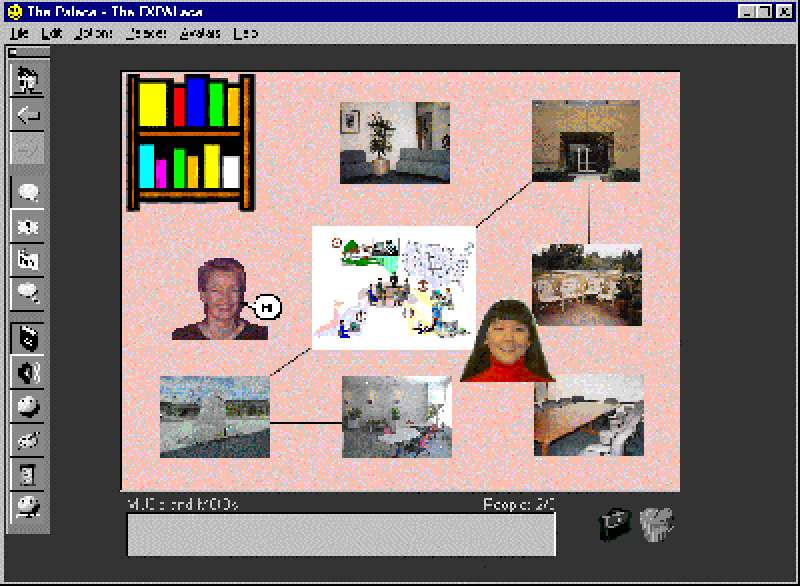
\includegraphics[width=0.4\linewidth]{figures/churchill_snowdon_cscw_vs_cve/A-room-created-using-The-Palace-with-two-avatar-embodiments}}
	\hfill
	\subfloat[CVE]{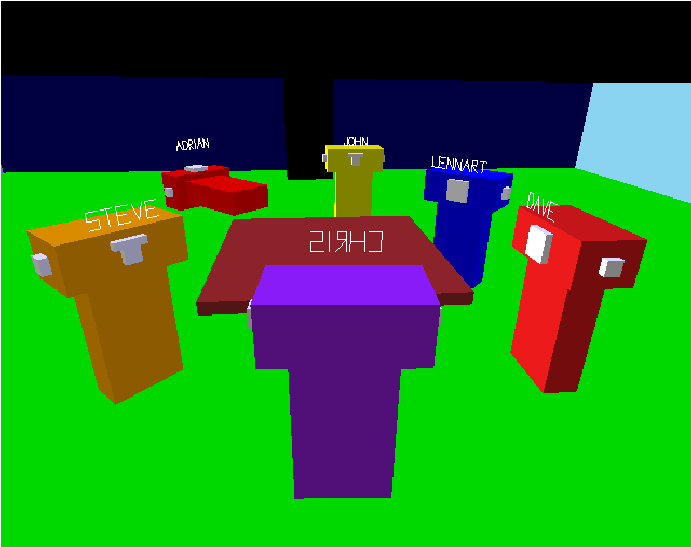
\includegraphics[width=0.4\linewidth]{figures/churchill_snowdon_cscw_vs_cve/Embodiments-in-MASSIVE-1}}
	\hfill
	\caption{Approaches to collaboration (Source: \cite{churchill_collaborative_1998})}
	\label{fig:approaches_to_collaboration}
\end{figure}

%[immersive CVE - greenwald cocoverse]
The next leap in digital collaboration was initiated with the introduction of the first generation \gls{vr} setups from Oculus Rift and HTC Vive. Their sub-millimeter tracking of head and hand-held controllers, high-resolution, high fidelity and wide field-of-view displays eased the problem of foreign interface  requiring high attention load, the initial reason why \gls{cve}s found much broader application in gaming, than in distributed workspaces. More detail on the history of the \gls{cve}s from the introduction to the topic by Churchill and Snowdon to the current day \gls{hmd}s for immersive \gls{vr} can be found in \cite{greenwald_technology_2017}.

\paragraph{Terminology}
To disambiguate the further discussion in this thesis, I will use the following terminology in this thesis: simply "\gls{vr}" will refer to the experiences through Oculus Rift-like mediums; "surround-screen \gls{vr}" will imply the use of surround-screen displays instead of tracked \gls{hmd}s to deliver the \gls{vr} experience; "\gls{ve} application" will refer to less immersive desktop \gls{vr} applications (see \cite{churchill_collaborative_1998}, Example Projects section). 
To follow the definition by \cite{jr_3d_2017}, when talking about collaboration, "\gls{cve} application" and "collaborative \gls{vr}" will correspond to the collaborative counterparts of the \gls{ve} application and \gls{vr}.
The term "digital collaboration" will refer to all the different types of collaboration through a digital medium: \gls{cscw}, gls{cve}, collaborative \gls{vr}, etc.
% TODO: can I introduce the new acronym "CVR"? Is it smart, considering no one is using it or will be searching for it.

\paragraph[Bridge]{}
The next chapter we will explore the realm of perception, specifically, the properties and applications of auditory information during digital collaboration.

\begin{comment}

\begin{figure}
	\centering
	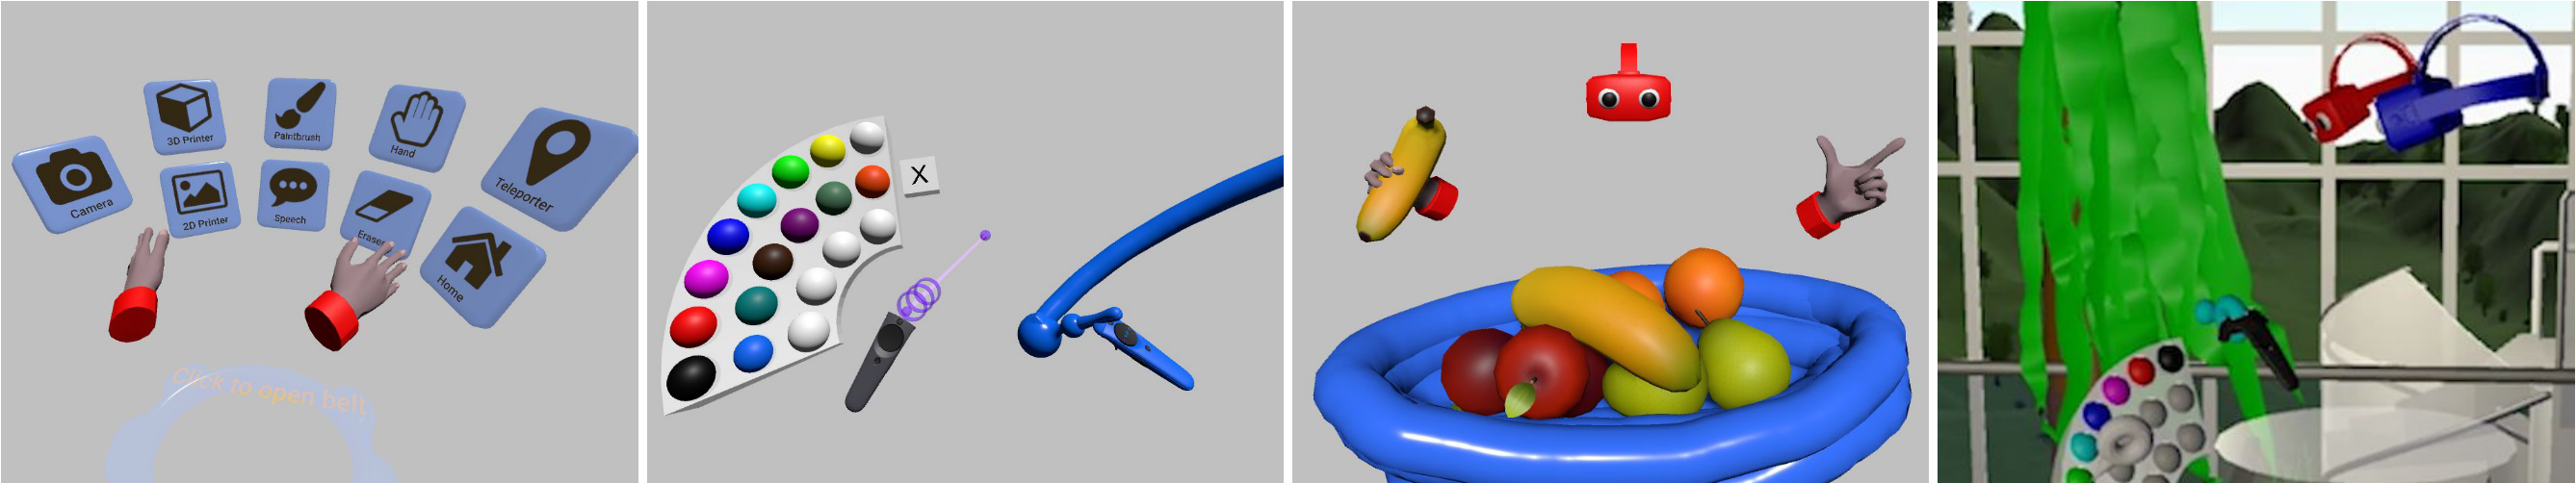
\includegraphics[width=0.7\linewidth]{figures/Cocoverse}
	\caption{CocoVerse, environment affordances and avatars (Source: \cite{greenwald_cocoverse_nodate})}
	\label{fig:cocoverse}
\end{figure}

\paragraph[Related Work]{}
We will now take a look at the some of the problems that were appraoched in the domain of digital collaboration.

% Interactions and navigation // THis is more a single-player problem
% Greenspace II
Some collaborative projects address the question of interactions with shared artifacts. From the earlier studies, \cite{davidson_greenspace_1996} present an immersive \gls{vr} system with 6 \gls{dof} tracked head and hand movements that facilitates design review and discussion of the architectural design decisions. This was much an exploratory study, where participants got to explore the design of a 3D environment in an interactive fashion. The authors report their findings on the navigation, communication, manipulation and some social affordances of the resulting application.
% Lena
\cite{lena_real-time_nodate} presents a research into what constitutes an interactions in \gls{vr} and utilizes the findings in the \gls{cdp} project to connect two "different realities": an interactive table computer and a CAVE-environment. Intentional non-verbal communication and embodiment are also explored.

% Presence
% CocoVerse
Next popular topic of research is the different types of presence, also described as a feeling of "being there".
Greenwald et al. (\cite{greenwald_cocoverse_nodate}, \cite{greenwald_investigating_2017}, \cite{greenwald_technology_2017}) are exploring the utility of shared immersive \gls{vr} for collaborative learning and co-operation. Authors present a system that is the first of its kind in the research community multi-user framework for collaboration and co-creation, CocoVerse (Fig. \ref{fig:cocoverse}). The topics addressed are: social presence (the quality of the medium in convincing users in the salience of the others, present in the same \gls{ve}), co-presence (psychological and emotional interactions between the users), embodiment (how users are represented), as well as non-verbal communication (i.e. through gestures).
Even though, it is already closer to our initial problem formulation, this stream of research focuses mostly on the phase where users' attention is equally engaged on the same subject.

% Awareness
\cite{gutwin_descriptive_2002} split a collaborative situation into two parts: the domain task and the collaborative part. Ammi and Katz, in their study on communication via audio and haptic feedback in abstract and non-visual environments, prior to implementation, derive requirements to the individual (domain) and collaborative parts of the application \cite{ammi_intermodal_2015}. The former include the concept of \gls{sa}, and the later consists of process and \gls{wa}.
% Situation & Workspace awareness differences
\gls{sa} is defined by Endsley as: "the perception of the elements in the environment within a volume of time and space, the comprehension of their meaning, and the projection of their status in the near future" \cite{endsley_situation_1988}. In-fact, \gls{wa} is a special type of \gls{sa} in shared workspaces. The first difference is that the focus of the \gls{sa} on the domain task only is extended with the focus on collaborative task. Secondly, the extreme flow of information that is typical for \gls{sa} due to its roots in the jet fighter simulations, is reduced in volume to match the use case of shared collaboration between colleagues. Main reason for this is, as authors put it: "sorting slides on a table does not seem very similar to air combat in a jet fighter" \cite{gutwin_descriptive_2002}.

% Similaritites
The part that is similar about the two types of awareness, and that makes this topic interesting in the context of current thesis, is that in both cases users are unable to gather the information they need. If, in case of a jet fighter simulation, the pilot is simply overwhelmed by the sheer volume of the information presented, then in the sorting slides task the users is failing to gather information due to the fact that the system does not present them with adequate awareness information by default.

% Workspace awareness framework: types of communication
The authors go ahead and introduce a descriptive framework to help groupware
designers determine what types of awareness presentations to include in their systems, and allow the comparison of the systems based on the extent to which they promote \gls{wa}.
The framework consists of three parts:
\begin{description}
	\item[Part I] What information makes up \gls{wa}?
	\item[Part II] How is the \gls{wa} information gathered?
	\item[Part III] How is \gls{wa} used in collaboration?
\end{description}

The second part of the framework provides insights about the different sources of \gls{wa} information: 
\begin{enumerate}
	\item Bodies and consequential communication;
	\item Artifacts and feedthrough;
	\item Conversation, gesture, and intentional communication.
\end{enumerate}
While 1 and 3 can be summarized as non-intentional and intentional communication, feedthrough is a mechanism of interest for our purposes, as it implies that artifacts (objects in the \gls{ve}) give off information (audio, visual, etc.) when manipulated, which simultaneously serves as a feedback to the person performing the manipulation and as a notification to the others present in the workspace.
% Gutwin_chalk_2011
The authors utilize this mechanism in their study on the use of synthesized audio to promote to promote \gls{wa} in a shared chalkboard application \cite{gutwin_chalk_2011}. In the systems, users are tasked with tracing a 2D shape (i.e. an outline of a ship), which is accompanied with an auditory feedback. There are two types of users in this environment - the real one (participant) and the simulated (user agent). The later is responsible for drawing shapes in the off-screen part of the workspace, while the former has two tasks - the primary and secondary. The primary task is to trace a given shape, and the secondary is to report that they noticed changes to the environment caused by the user agent. Among other topics, the authors explore the effect different awareness presentations and their combinations (type of auditory feedback, availability of the minimap of the environment, workspace clutter, and attention load) have on the \gls{wa}. They report a substantial increase in awareness due to the use of audio to convey information.
\begin{figure}
	\centering
	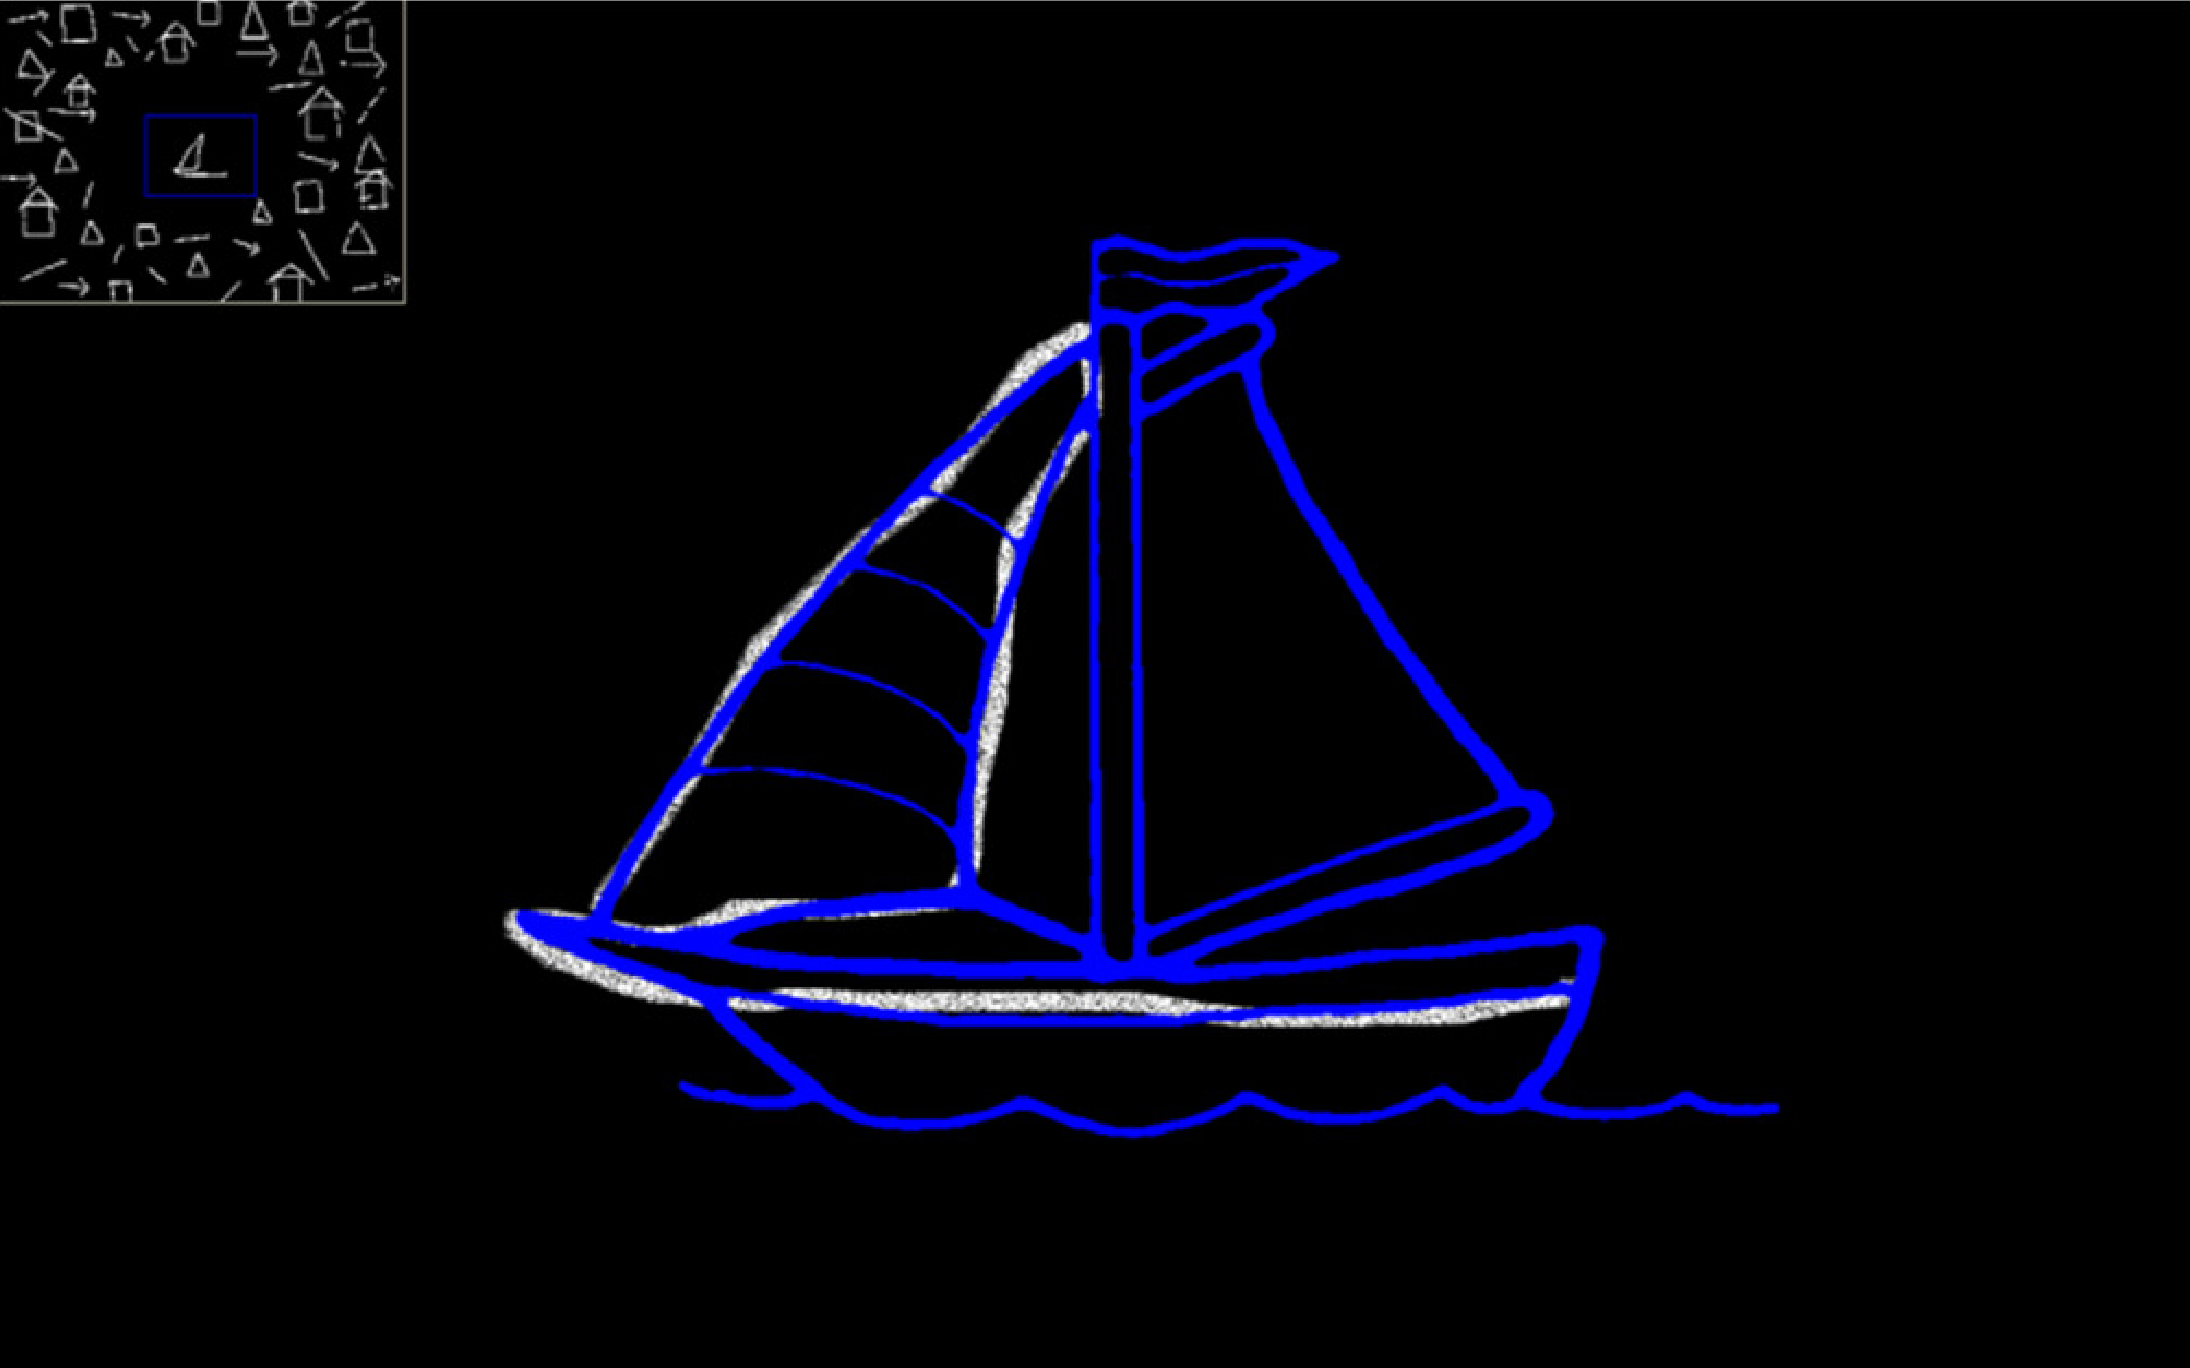
\includegraphics[width=0.7\linewidth]{figures/gutwin_chalk_2011}
	\caption{Shared chalkboard application, tracing shape and minimap (Source: \cite{gutwin_chalk_2011})}
	\label{fig:gutwinchalk2011}
\end{figure}

In the next chapter we take a closer look at some of sound properties that can be utilized our application to counter the unexpected changes to the environment and enhance the \gls{wa}.

\end{comment}

\begin{comment}


% Gutwin
Gutwin and Greenberg explore the effects of synthesized sound in a shared chalkboard \gls{cscw} on the \gls{wa} ("the up-to-the-moment understanding of another person’s interaction with a shared workspace"). In this system two users are sharing a 2D workspace (a chalkboard). One user was real (participant) and another was simulated (agent). The agent would draw in an off-screen part of the workspace, this activity was accompanied by a synthesized sound. The real user had two tasks - primary and secondary. The former was to trace a given 2D shape (i.e. an outline of a ship) in their part of the shared workspace, and the later was to indicate whether they noticed the changes caused by the agent. % TODO: I don't look so deep into other studies
The authors study the extent of the ability of auditory cues to signal changes in the workspace, in comparison and in combination with a minimap.

% Ammi & Katz
\cite{ammi_intermodal_2015} study the application of abstract and non-visual \gls{vr} environments in the context of improving communication. The system facilitates a collaborative search of targets with the help of audio and haptic feedback. The authors work out a specification for both the individual and the collaborative aspects of the task. The concept of \gls{sa} is used to address the former, and workspace and process awarenesses - the later.

As we have seen, even in the fields of \gls{cscw} and \gls{cve}, a broad range of topics can be addressed with respect to collaboration..
We have viewed non-visual, 2D, immersive \gls{vr} environments 
These are only some..
We will now take a closer look at the awareness approach, as it provides us with..
% Intentional and unintentional communication? Communication with aware person and unaware person - Nah, the difference is in the type of the task that is being conducted. In gutwin the domain task is being explored, while the others explore the collaborative part.

Collaboration can be approached in different ways, depending on the task at hand. More traditional approach is with \gls{cscw} systems, it works well when the task is routine and just requires either information exchange, or an execution of a pre-defined task \cite{churchill_collaborative_1998}. For more creative and non-trivial tasks, which can be obscured by enforcing a certain workflow early-on, an approach using \gls{cve} is more appropriate.

\paragraph{}
% CVEs
One of the origins of \gls{cve}s is the field of \gls{vr}. This is mostly due to the aim  to allow users creative freedom, and reduce the learning curve by providing an intuitive interface. The task of a \gls{cve} is to facilitate communication and collaboration. They allow synchronous and asynchronous task execution, and provide the support for real-time sharing of visual artifacts \cite{churchill_collaborative_1998}.

\subparagraph{}
% Cocoverse, Greenwald - first system of this kind in the research community
A good and concise review of the history of the \gls{cve}s can be found in \cite{greenwald_technology_2017}. The state of art in the area of CVEs was reached by one of the authors, in \cite{greenwald_cocoverse_nodate} and \cite{greenwald_investigating_2017} he presents CocoVerse - a shared immersive \gls{vr} environment for local collaboration and co-creation (Fig. \ref{fig:cocoverse}).

\begin{figure}
	\centering
	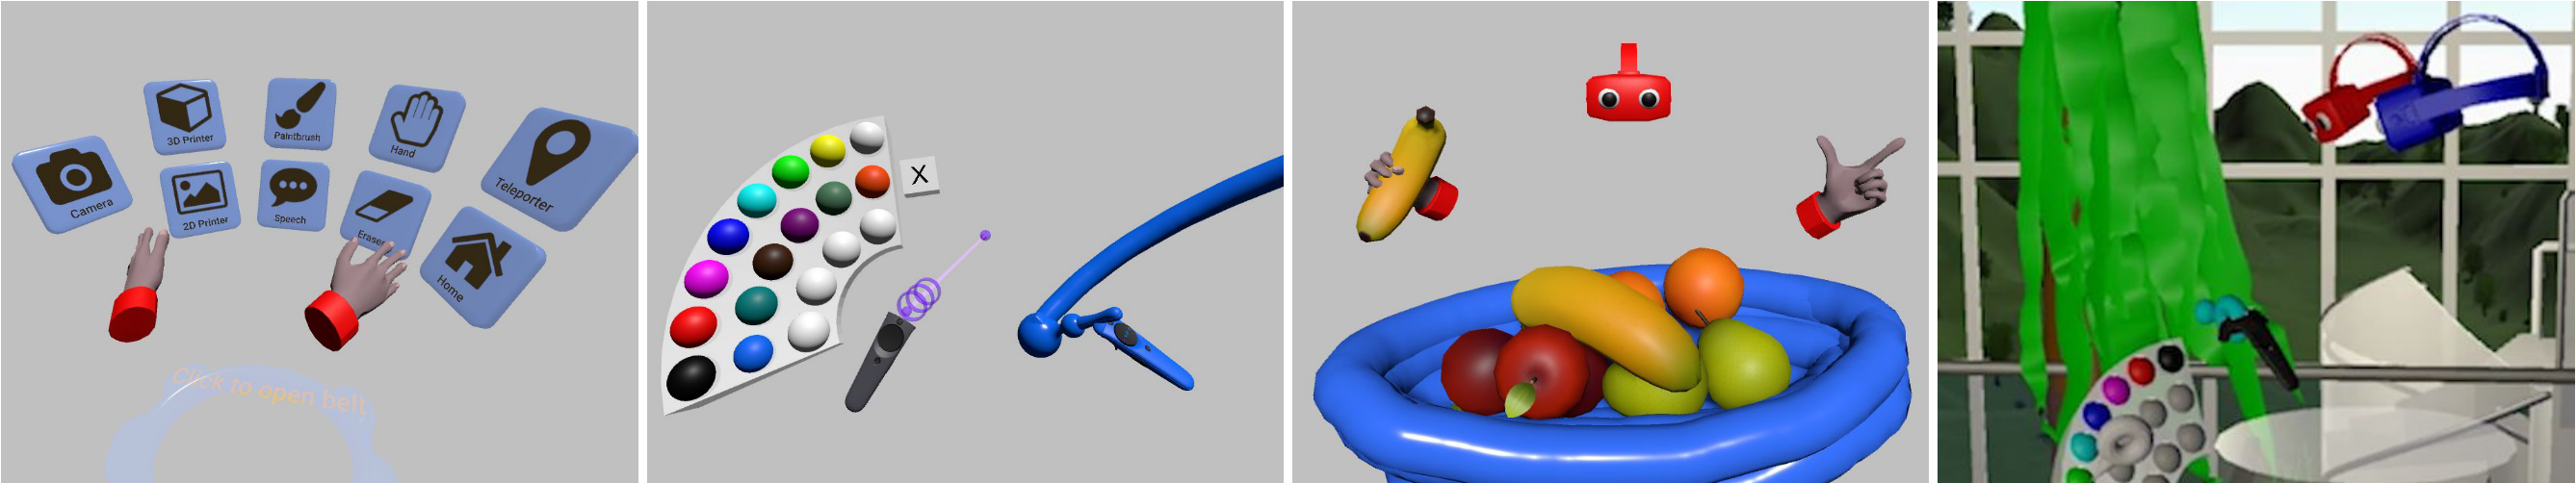
\includegraphics[width=0.7\linewidth]{figures/Cocoverse}
	\caption{CocoVerse, environment affordances and avatars (Source: \cite{greenwald_cocoverse_nodate})}
	\label{fig:cocoverse}
\end{figure}

%% What they explored, their focus and discoveries
%%% Goals
Authors' main research direction is communication, collaboration, and learning in \gls{vr}. As the field of immersive \gls{vr} is relatively young, one of the main goals of those projects was to explore the feasibility and utility of such setup, and pilot methodologies for studying behavior in this setting (\cite{greenwald_investigating_2017}). The utility was analyzed by comparing different activities in the 2D viewing mode (via a monitor) and as the immersive 3D experience.

%%% Setup/system
The system is a room-scale shared immersive \gls{vr} experience, which allows users to synchronously manipulate the environment with a set of hand-based tools (create 3D drawings, communicate via rough hand gestures, etc.). CocoVerse also lets the users know where others are looking, by providing them with minimalistic avatars that convey the gaze direction. Users require either a \gls{hmd} and a pair of 6 \gls{dof} controllers to use the system in the immersive mode, or simply a PC to participate in the 2D mode.

%%% Focus and the results
Authors report the overall success and promise of such setups as an engine for learning and creativity. They further review, how the sense of social presence is influenced by the complexity of avatars and high movement realism. \cite{greenwald_investigating_2017} proposes guidelines for deciding on the level of sophistication of the embodiment based on the type of experience that is being digitalized.

% Concise: what other CVE projects addressed.
Among other CVEs that were explored, \cite{lena_real-time_nodate} proposes a system, which connects two different mediums (an interactive table computer, and a CAVE-environment), and focuses on the way to develop consistent interactions across the environment. % TODO: more (e.g. Kulik)

% Conclusion: something else is needed
Generally, it seems that the focus of the modern \gls{cve} projects is more on exploring the aspects of the intentional communication and interactions, where users are always aware of each other during the collaboration task. I our case, the focus should be more on consequential communication, which arises as a result of user's actions.

\subparagraph[CSCW]{}
% CSCWs
We will now turn to the field of \gls{cscw}, which is regarded by \cite{churchill_collaborative_1998} as the main way to approach the automation of the collaborative work, before the paradigm shift towards \gls{cve}s. \gls{cscw} applications also provide distributed access to a shared context. However, unlike \gls{cve}s, these applications provide a less malleable environment that is restricted by requirements of a certain workflow. Examples of \gls{cscw} applications include: emailing software, project management and conferencing tools, shared calendars and drawing tools, etc.

% Chalkboard, Gutwin
A notable work from the field of \gls{cscw} is the study presented in \cite{gutwin_chalk_2011}. The authors study the use of auditory cues to promote the up-to-the-moment understanding of another person’s interaction with the shared chalkboard application, or as they call it, the "Workspace Awareness" (WA) \cite{gutwin_descriptive_2002}. % TODO: I use the same quote in the Awareness chapter. Change.

%% What they explored, their focus and discoveries
%%% Goals
Two main goals of the study were to figure out "How much information can sound convey?" and the effectiveness of audio awareness in a \gls{cscw} application.

%%% Setup/system
The system is a 2D shared drawing application with one real (participant) and one simulated user (called an \textit{agent} in the \gls{cve} terminology). The participant has two tasks, primary and secondary. The primary task was to trace a given 2D shape (Fig. \ref{fig:gutwinchalk2011}), and the secondary was to keep track of what is happening in the shared workspace. When a participant and the agent drew, the system would emit a spatialized sound of chalk writing on a chalkboard (at a lower volume for the participant's actions). An additional way to monitor the shared environment, or as authors call it - a type of awareness presentation, was a minimap (what authors call a \textit{radar}), which showed the complete environment and the local chunk a participant was working in (indicated with a blue rectangle on the minimap).
% The workspace is seen in the figure
% Different awareness presentations - auditory and minimap
% Varying difficulty of the tracing shape

\begin{figure}
	\centering
	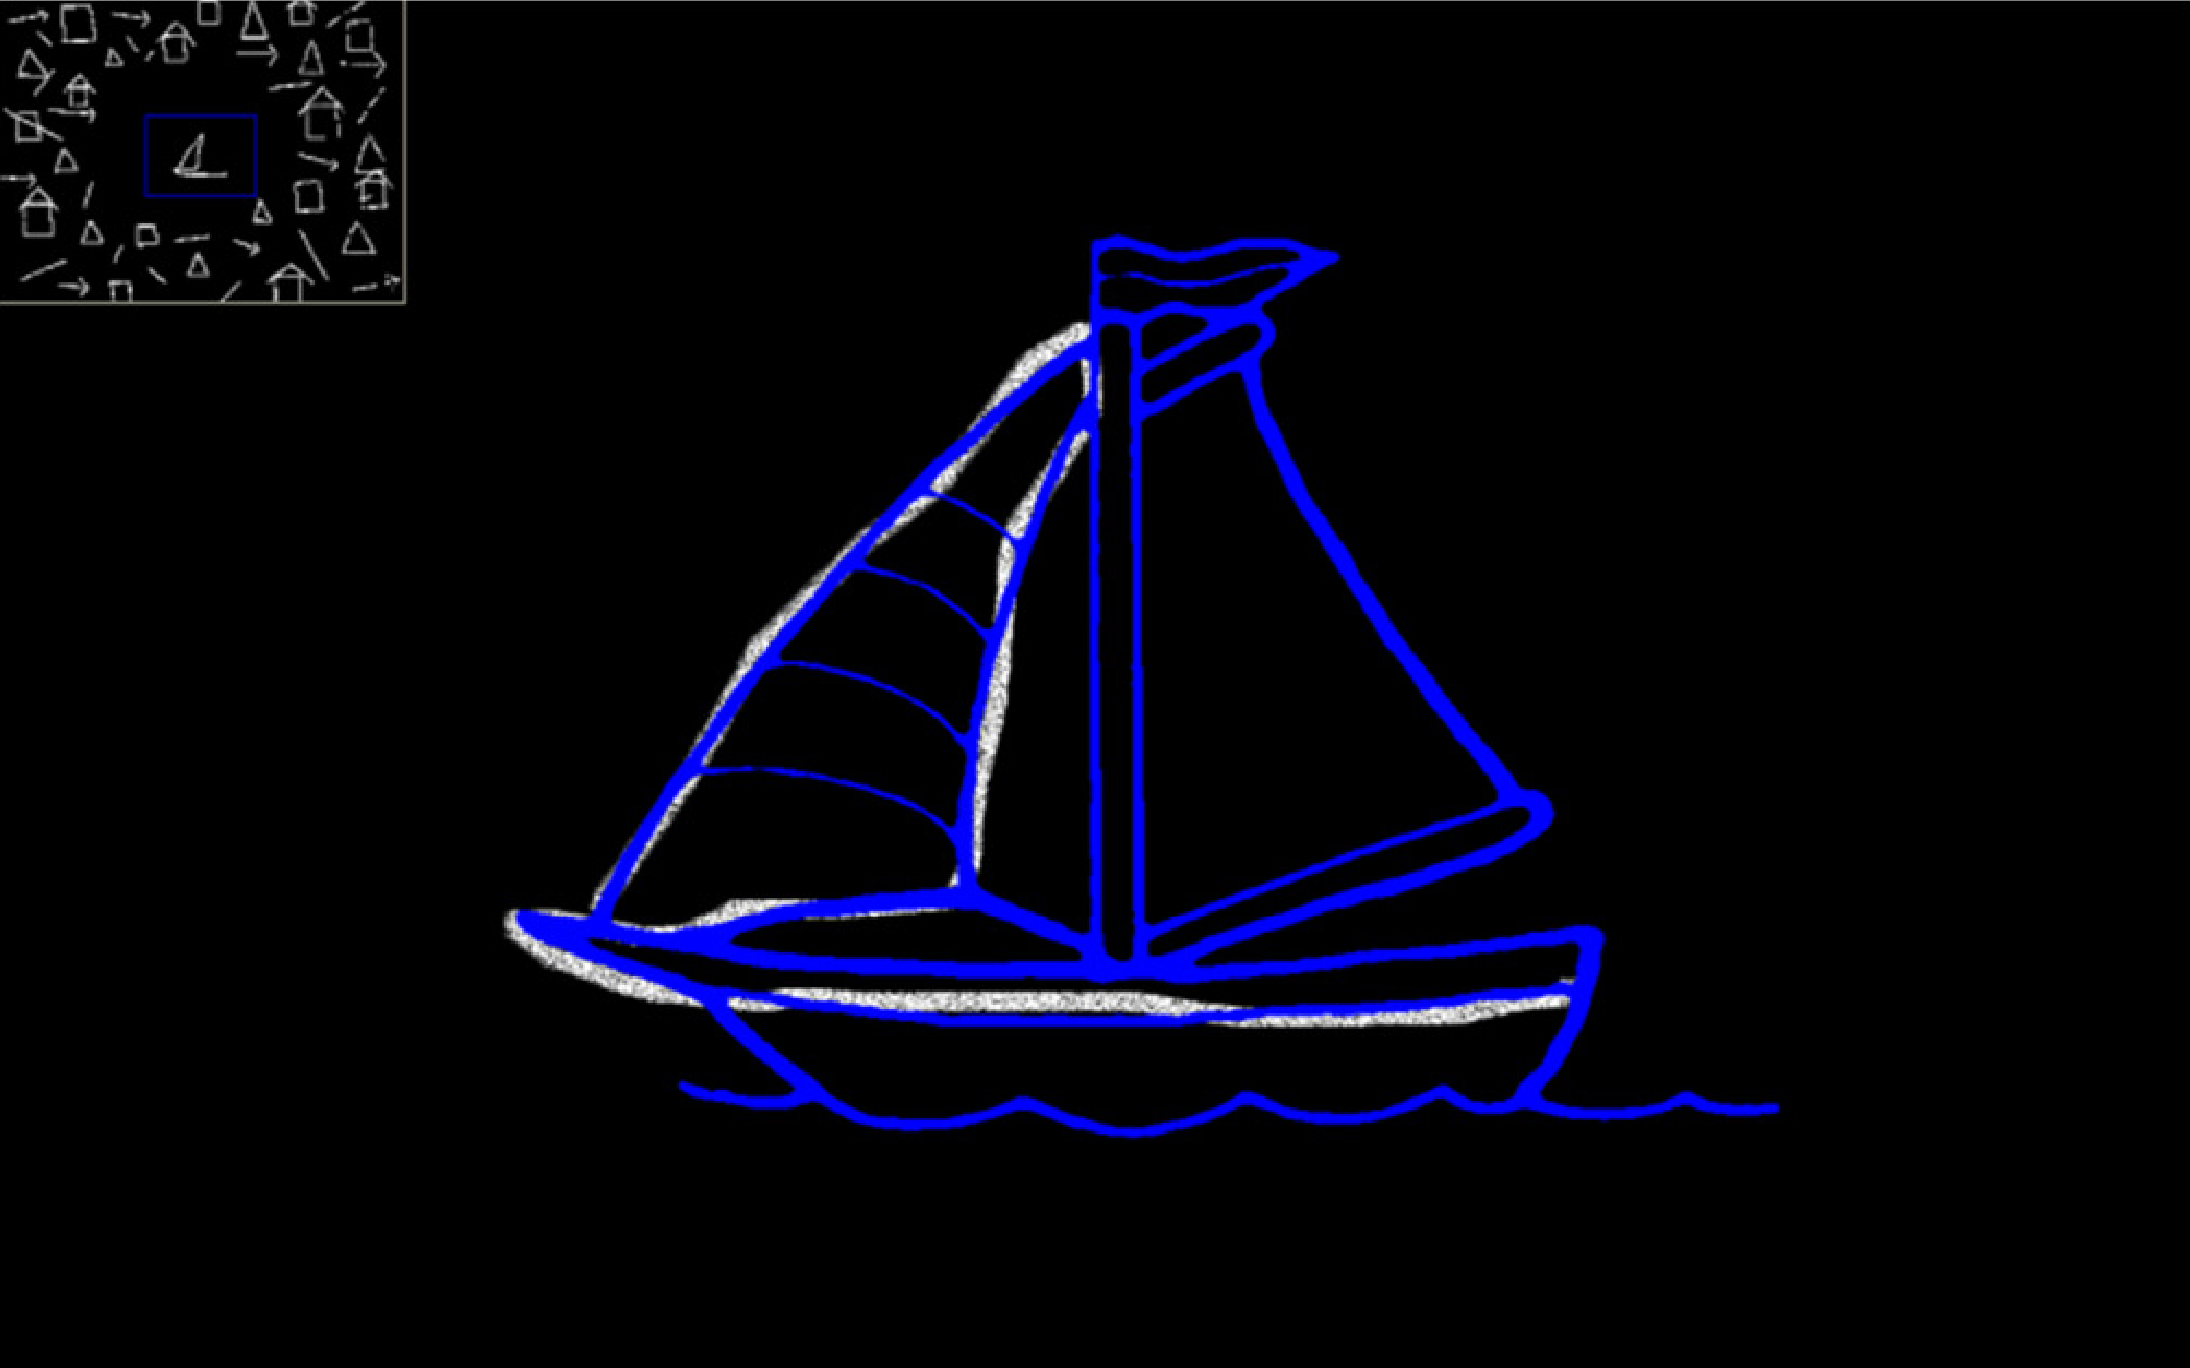
\includegraphics[width=0.7\linewidth]{figures/gutwin_chalk_2011}
	\caption{Shared chalkboard application, tracing shape and minimap (Source: \cite{gutwin_chalk_2011})}
	\label{fig:gutwinchalk2011}
\end{figure}


%%% Focus and the results
One of the characteristics of the \gls{wa} is that it is a peripheral (or a secondary) task by nature \cite{gutwin_descriptive_2002}, % TODO: I might be using the same quote in the Awareness chapter. Change.
as such, \cite{gutwin_chalk_2011} attempt to keep participant's attention on the main task by varying the difficulty of the tracing activity: the tracing shape was made to oscilate occasionally. Authors also study the effect of the workspace clutter, the size of the minimap, the type of auditory cues, and the awareness presentation on the \gls{wa}.

The authors report significant improvements to the group awareness in cases, where it is hard to attend to the visual displays, or the line of sight is obscured. Additionally, they provide their thoughts with regards to how and why the audio awareness helps in the collaborative scenarios, as well as the possible limitations of its application.

\paragraph[Bridge]{}
The approach used in \cite{gutwin_chalk_2011} is based on their previous work on the topic of \gls{wa} \cite{gutwin_descriptive_2002}.
Next, we are going to take a closer look at the awareness approach % TODO: did I define it?
, its history, and how it aids the design of the groupware systems. 


\end{comment}





\begin{comment}
% Intro: Introduce what this whole chapter is about

This chapter is going describe the ?status quo of the Collaborative Virtual Environments, highlight the state of art, and the experiment on the Workspace Awareness that the practical part of this thesis took as the base.

\section{Status quo}
.. Like theory part
Define CVE, Groupware, and cooperation levels
% Talk about users and agents, cause I mention it in the experminets chapter.

\section{Related projects}
Mention some projects that are related, but won't be discussed in the detail in this work. The purpose of this subsection is to provide an overview of the current state of the groupware/collaborative software systems.
Lena
® Provides a good overview of the Collaboration and interaction in similar projects
® Focuses more on interactions …
Greenspace II
® A related work from the architectural filed
® Morally aged, Greenwald uses some findings from it
[some other works]

\section{State of art: Multi-User Framework for Collaboration and Co-Creation in Virtual Reality}
§ In this section I will discuss the work I found, which serves as the state of art for current development of Collaborative Virtual Environments (CVEs) - Multi-User Framework for Collaboration and Co-Creation in Virtual Reality (Greenwald et al. 2017).


\section{Parent/precursor/foundation work: The Effects of Dynamic Synthesized Audio on Workspace Awareness in Distributed Groupware}
§ Introduce Gutwin et al. 2011 work on The Effects of Dynamic Synthesized Audio on Workspace Awareness in Distributed Groupware (Chalk Sounds)

Goals

Setup/system
® …
® 

\begin{table}[]
	\begin{tabular}{|l|l|}
		\hline
		Number of people                                                                                  & Conceptually, multiuser                                                                                                \\ \hline
		Medium                                                                                            & PC with an interactive display for drawing                                                                             \\ \hline
		\begin{tabular}[c]{@{}l@{}}Affordances \\ (TODO: make it correspond to WA framework)\end{tabular} & \begin{tabular}[c]{@{}l@{}}Manipulation: 2D drawing, self-report\\ Communication: auditory icons, minimap\end{tabular} \\ \hline
		?Cooperation level                                                                                & Conceptually, 3.2                                                                                                      \\ \hline
		Locality                                                                                          & Shared physical space and remote collaboration                                                                         \\ \hline
	\end{tabular}
\end{table}

Focus and the results
\end{comment}
